% "{'classe':('PSI'),'chapitre':'dyn_inertie','type':('cours'),'titre':'Caractérisation inertielle des solides', 'source':' ','comp':['B2-10',],'corrige':True}"
\setchapterimage{Fond_CIN.png}
\setchapterpreamble[u]{\margintoc}
%\setcounter{chapter}{1}

\chapter{Caractérisation inertielle des solides}

\marginnote[2cm]{
\UPSTIcompetence[2]{B2-10}
}

\marginnote[3cm]{\textbf{Emilien Durif}, \textit{Introduction à la dynamique des solides}, Lycée La Martinière Monplaisir, Lyon.}
\marginnote[4cm]{\textbf{Florestan Mathurin}, \textit{Géométrie des masses}, Lycée Bellevue, Toulouse \url{http://florestan.mathurin.free.fr/}.}
\marginnote[5cm]{\textbf{Robert Papanicola}, \textit{Opérateurs d'inertie}, Lycée Charlemagne, Paris, \url{http://sciences-indus-cpge.papanicola.info/}.}


\begin{marginfigure}[6.5cm]
\centering
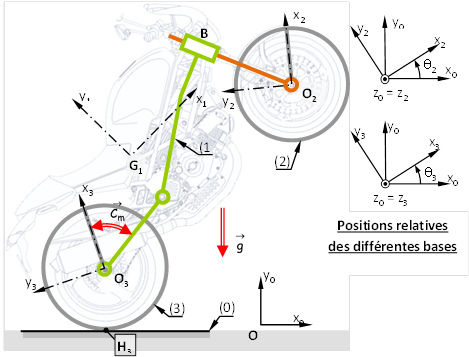
\includegraphics[width=4cm]{fig_01}
\caption{Toupie}
\end{marginfigure}


\begin{marginfigure}[10.5cm]
\centering
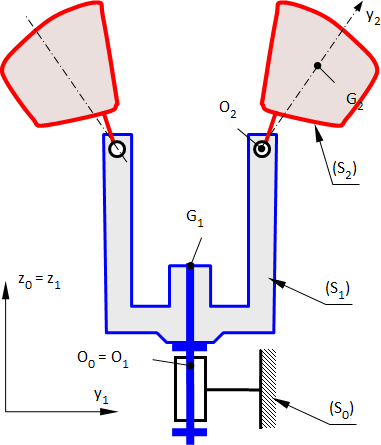
\includegraphics[width=4cm]{fig_02}
\caption{Volants d'inertie d'un vilebrequin}
\end{marginfigure}



\section{Masse et centre de masse (centre d'inertie)}
\subsection{Définitions}
\begin{defi}[Masse d'un solide indéformable]
On peut définir la masse totale d'un solide $S$ par : $M=\int\limits_{P\in S} \,\dd m$. Si de plus l'ensemble est fait d'un matériau homogène de masse volumique $\mu$, on a $M=\mu \int\limits_{P\in S} \dd V$. \end{defi}


\begin{defi}[Centre d'inertie d'un solide]
La position du centre d'inertie $G$ d'un solide $S$ est définie par $\int\limits_{P\in S} \vect{GP} \dd m = \vect{0}$.
\end{defi}

Pour déterminer la position du centre d'inertie d'un solide $S$, on passe généralement par l'origine du repère associé à $S$. On a alors 
$\int\limits_{P\in S} \vect{GP} \, \dd m=\int\limits_{P\in S} \left(\vect{GO}+\vect{OP}\right) \dd m = \vect{0} 
\Leftrightarrow \int\limits_{P\in S} \vect{OG} \,\dd m =\int\limits_{P\in S} \vect{OP} \,\dd m
\Leftrightarrow  M\vect{OG} =\int\limits_{P\in S} \vect{OP} \,\dd m$.

\begin{methode}[Coordonnées du centre d'inertie]
Pour déterminer les coordonnées $\left(x_G,y_G,z_G\right)$ du centre d'inertie $G$ du solide $S$ dans la base $\repere{O}{x}{y}{z}$, on a donc :
$$
\left\{
\begin{array}{l}
M x_G =\mu \int\limits_{P\in S} x_P \,\dd V \\
M y_G =\mu \int\limits_{P\in S} y_P \,\dd V \\
M z_G =\mu \int\limits_{P\in S} z_P \,\dd V \\
\end{array}
\right. \quad \text{avec }\dd V \text{ volume élémentaire du solide $S$.}
$$ 

Pour simplifier les calculs, on peut noter que le centre d'inertie appartient au(x) éventuel(s) plan(s) de symétrie du solide.
\end{methode}

\begin{remarque}
Centre d'inertie et centre de gravité sont confondus lorsque le champ de pesanteur est considéré comme uniforme en tout point de l'espace. 
\end{remarque}

\subsection{Centre d'inertie d'un ensemble de solides encastrés entre eux}
\begin{methode} [Barycentre d'un assemblage]
Soit un solide composé de $n$ solides élémentaires dont la position des centres d'inertie $G_i$ et les masses $M_i$ sont connues. On note $M=\sum\limits_{i=1}^{n}M_i$.  La position du centre d'inertie $G$ de l'ensemble $S$ est donné par :
$$\vect{OG}=\dfrac{1}{M}\sum\limits_{i=1}^{n}M_i \vect{OG_i} .$$

\end{methode}


\subsection{Méthode pour déterminer le centre d'inertie d'un solide \cite{2}}
\begin{center}
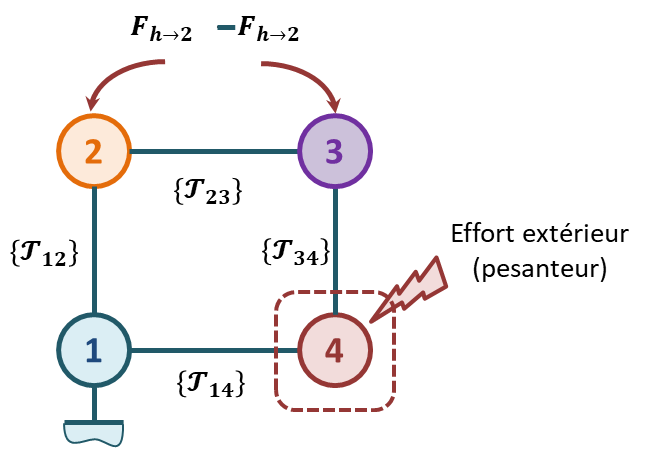
\includegraphics[width=.55\linewidth]{fig_04}
\end{center}

\section{Matrice d'inertie d'un solide}
\subsection{Opérateur et matrice d'inertie}

\begin{defi}[Opérateur d'inertie]
Soient : 
\begin{itemize}
\item un solide $S$ de masse $m$ en mouvement par rapport à un repère $\mathcal{R}_0=\repere{O_0}{i_0}{j_0}{k_0}$;
\item $\mathcal{R}_S=\repere{O}{i}{j}{k}$ le repère lié au solide $S$;
\item $P$ un point de $S$ tel que $\vect{OP}=x_p\vect{i}+y_p\vect{j}+z_p\vect{k}$;
\item $\vect{u}$ un vecteur unitaire lié au solide $S$ tel que $\vect{u}=u_x \vect{i}+u_y \vect{j}+u_z \vect{k}$.
\end{itemize}

On appelle opérateur d'inertie l'application linéaire définie par :
$$
\vect{u} \rightarrow \vect{J_{\left(O,S\right)}\left(\vect{u}\right)} 
= \int\limits_{S} \vect{OP}\wedge \left(\vect{u}\wedge \vect{OP}\right)\,\dd m
$$

On appelle matrice d'inertie du solide $S$ en $O$, $\inertie{O}{S}$, l'image de cette application linéaire : $\vect{J_{\left(O,S\right)}\left(\vect{u}\right)}  = \inertie{O}{S} \vect{u}$.
 
\end{defi}

\begin{defi}[Matrice d'inertie]
La matrice d'inertie s'écrit ainsi : 
$$
\inertie{O}{S}=\matinertie{\int\limits_{S} \left(y_p^2 + z_p^2 \right)\,\dd m}{\int\limits_{S} \left(x_p^2 + z_p^2 \right)\,\dd m}{\int\limits_{S} \left(x_p^2 + y_p^2 \right)\,\dd m}{-\int\limits_{S} \left(y_pz_p\right)\,\dd m}{-\int\limits_{S} \left(x_pz_p\right)\,\dd m}{-\int\limits_{S} \left(x_py_p\right)\,\dd m}{\mathcal{R}_S}$$
$$=\matinertie{A}{B}{C}{-D}{-E}{-F}{\mathcal{R}_S}
.$$

On appelle moments d'inertie par rapport aux axes $\axe{O}{{x}}$, $\axe{O}{{y}}$ et $\axe{O}{{z}}$  les termes $A$, $B$ et $C$. 

On appelle produit d'inerties par rapport aux axes $\axe{O}{{y}}$ et $\axe{O}{{z}}$,  $\axe{O}{{x}}$ et $\axe{O}{{z}}$,  $\axe{O}{{x}}$ et $\axe{O}{{y}}$ les termes $D$, $E$ et~$F$.
\end{defi}

\begin{prop}

\begin{itemize}%[label=\ding{112},font=\color{bleuxp}] 
\item La matrice d'inertie est une matrice symétrique. Il existe une base dans laquelle elle est diagonalisable. Cette base est appelée base principale d'inertie. 
\item Si $\left(O,\vect{x},\vect{y} \right)$ est un plan de symétrie du solide, $D$ et $E$ sont nuls.
\item Si $\left(O,\vect{z},\vect{x} \right)$ est un plan de symétrie du solide, $D$ et $F$ sont nuls.
\item Si $\left(O,\vect{y},\vect{z} \right)$ est un plan de symétrie du solide, $E$ et $F$ sont nuls.
\item Si un solide admet 2 plans de symétrie, alors $D$, $E$ et $F$ sont nuls. 
\end{itemize}

\end{prop}

\begin{marginfigure}
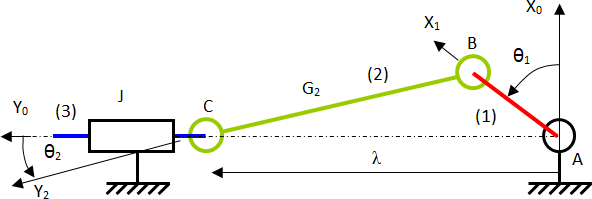
\includegraphics[width=.95\linewidth]{fig_03}
\end{marginfigure}


\begin{defi}[Moment d'inertie par rapport à un axe quelconque]
Le moment d’inertie caractérise la répartition de masse d’un solide autour d’un axe $\Delta$ $\left(O,\vect{u}\right)$. Plus la valeur
de l’inertie est grande plus il sera difficile de mettre en mouvement de rotation ce solide autour de
l’axe $\Delta$. 
On note $I_{\Delta}(S)$, le moment d’inertie du solide $S$ autour de l’axe $\Delta$. Son unité est en $\text{kg.m}^2$.

Si on connaît $\inertie{O}{S}$, alors $I_{\Delta}(S)=\vect{u}^\top\inertie{O}{S}\vect{u}$ avec $\vect{u}$ \textbf{vecteur unitaire}.
\end{defi}


\begin{remarque}
On a aussi : 
$$I_{\Delta}(S)=\int\limits_{S} d_{\Delta}^2 \dd m \quad \text{où } d_{\Delta} \text{ est la distance entre le point courant } P \text{ et l’axe }\Delta.$$

\end{remarque}

\subsection[Déplacement d'une matrice d'inertie]{Déplacement d'une matrice d'inertie -- Théorème de Huygens}

\begin{theoreme}[Théorème de Huygens]
Soit $S$ un solide de centre d'inertie $G$, de masse $m$, d'inertie $\inertie{G}{S}$ et d'inertie $\inertie{O}{S}$ avec $\vect{OG}=a\vect{x}+b\vect{y}+c\vect{z}$. Les matrices $\inertie{G}{S}$ et $\inertie{O}{S}$ exprimées dans la base $\mathcal{B}=\base{x}{y}{z}$ sont liées par : 
$$
\matinertie{A_O}{B_O}{C_O}{-D_O}{-E_O}{-F_O}{\mathcal{B}}
= \matinertie{A_G}{B_G}{C_G}{-D_G}{-E_G}{-F_G}{\mathcal{B}}$$
$$
+ \matinertie{m\left(b^2+c^2\right)}{m\left(a^2+c^2\right)}{m\left(a^2+b^2\right)}{-mbc}{-mac}{-mab}{\mathcal{B}}.
$$


Si le solide est modélisé par une masse ponctuelle $m$ en $G$ et si on souhaite connaître le moment d'inertie pour un point situé à une distance $d$ de $G$, on a $I=md^2$.

\end{theoreme}


\subsection{Changement de base de la matrice d'inertie}
\begin{defi}[Matrice de Passage]
On appelle $P_{12}$ la matrice de passage permettant de passer de la base $\mathcal{B}_1$ à la base $\mathcal{B}_2$. Cette matrice est constituée en colonnes des coordonnées des vecteurs de la base $\mathcal{B}_2$ écrits dans la base d'origine $\mathcal{B}_1$. On l'appelle aussi matrice de changement de base. Cette matrice est inversible.

Dans le cas des matrices de rotation, $P_{12}^{-1}=P_{12}^{\top}$.
\end{defi}

\begin{exemple}
Soit $\rep{1}\repere{O}{x_1}{y_1}{z}$ et $\rep{2}\repere{O}{x_2}{y_2}{z}$ avec
$\beta = \angl{x_1}{x_2}$. On a alors $\vect{x_2}=\cos\beta\vect{x_1}+\sin\beta\vect{y_1}$ et $\vect{y_2}=\cos\beta\vect{y_2}-\sin\beta\vect{x_2}$. En conséquences, $P_{12}=
\begin{pmatrix} 
\cos\beta & -\sin \beta & 0\\  
\sin\beta & \cos \beta & 0\\  
0 & 0 & 1\\  
\end{pmatrix}$.
\end{exemple}

\begin{resultat}
Pour passer $\inertie{A}{S}_{\mathcal{B}_1}$ de ${\mathcal{B}_1}$ et ${\mathcal{B}_2}$  de la on a $\inertie{A}{S}_{\mathcal{B}_2} = P_{12}^{-1} \inertie{A}{S}_{\mathcal{B}_1} P_{12} $.
\end{resultat}



\subsection{Détermination de la matrice d'inertie d'un solide \cite{2}}

\begin{center}
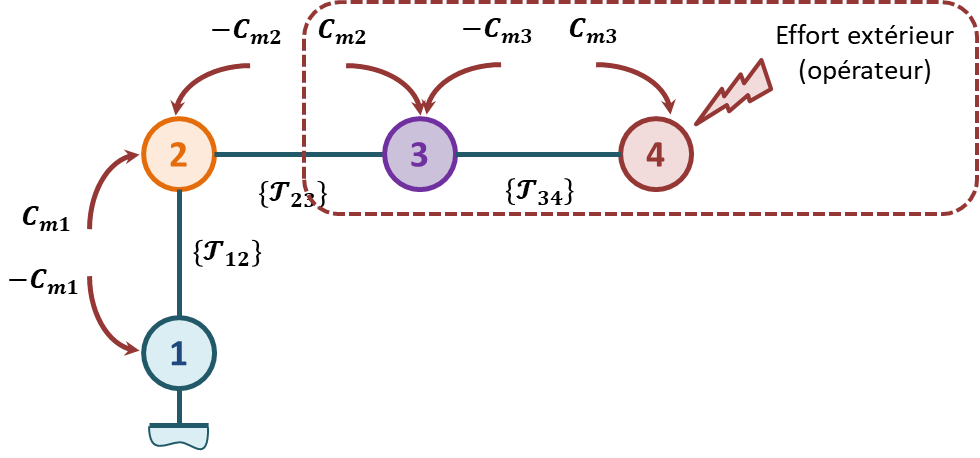
\includegraphics[width=.7\linewidth]{fig_05}
\end{center}
%\subsection{Compléments}

\subsection{Matrice d'inertie de solides usuels [3]}

\begin{table*}[!h]
\begin{center}
\begin{tabular}{ccc}
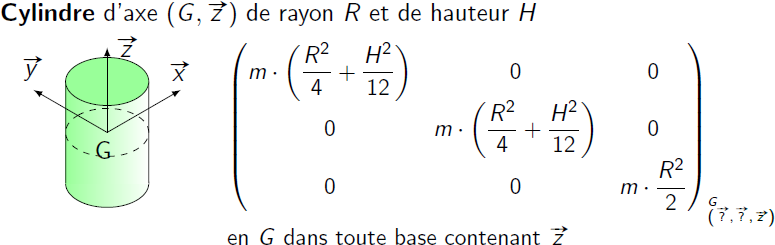
\includegraphics[width=7cm]{mat_01} & &
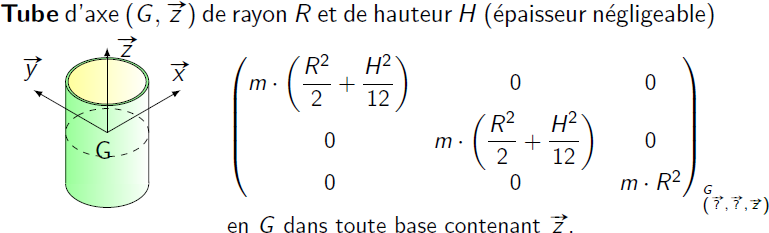
\includegraphics[width=7cm]{mat_02} \\ 
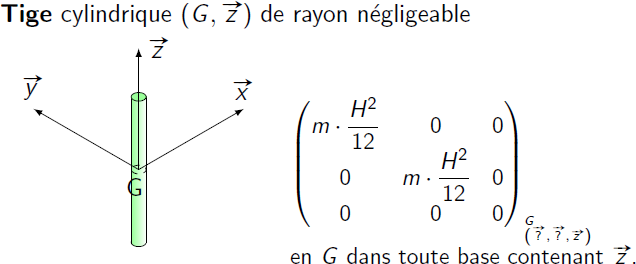
\includegraphics[width=7cm]{mat_03} & &
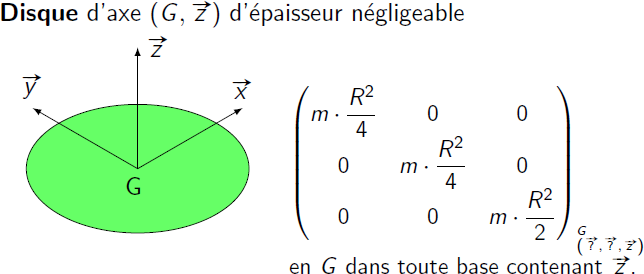
\includegraphics[width=7cm]{mat_04} \\ 
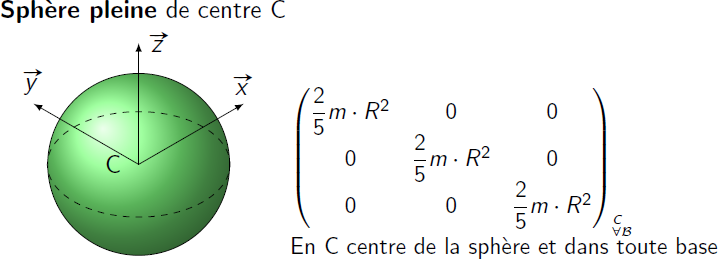
\includegraphics[width=7cm]{mat_05} & &
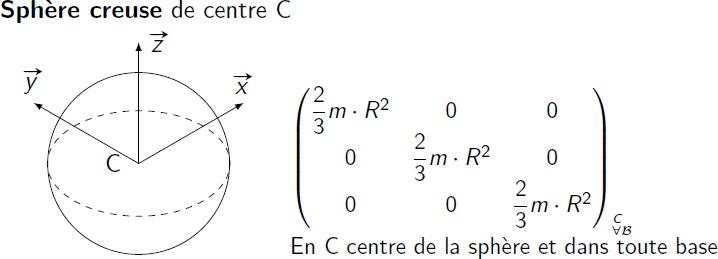
\includegraphics[width=7cm]{mat_06} \\ 
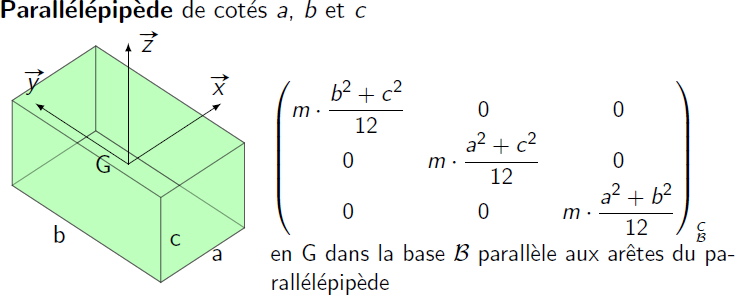
\includegraphics[width=7cm]{mat_07} & &
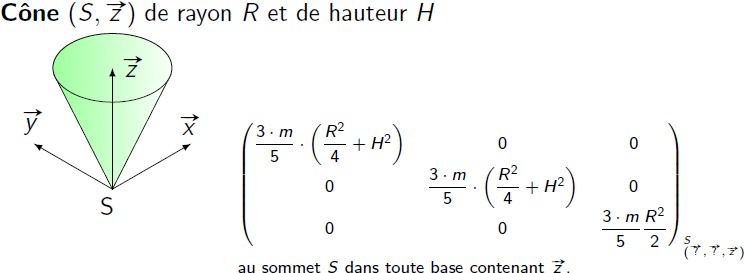
\includegraphics[width=7cm]{mat_08} \\ 
\end{tabular}
\end{center}
\end{table*}



